% -----------------------------------------------------------------
% Document class: Article
\documentclass[ a4paper, twoside, 11pt]{article}
\usepackage{../../../macros-general}
\usepackage{../../../macros-article}
% Number of the handout, quiz, exam, etc.
\newcommand{\numero}{01}
\setcounter{numero}{\numero}

% -----------------------------------------------------------------
\begin{document}
\allowdisplaybreaks

\begin{center}
\Large Mec\'anica Vectorial (MECG-1001): Trabajo Aut\'onomo \numero \\[2ex]
\small \textbf{Semestre:} 2017-2018 T\'ermino II \qquad
\textbf{Instructor:} Luis I. Reyes Castro \qquad
\textbf{Paralelo:} 08
\end{center}
\fullskip

% =============================================
\begin{problem}
Considere la llave curva mostrada en la figura de abajo. 
\begin{itemize}
\item \textbf{[2 Puntos]} Para el caso cuando $\alpha = 30\deg$ encuentre el momento que la fuerza $F$ ejerce sobre el perno en $O$. 
\item \textbf{[2 Puntos]} Encuentre el \'angulo $\alpha$ que maximiza el momento ejercido por la fuerza $F$ sobre el perno en $O$. 
\end{itemize}

\begin{figure}[htb]
\centering
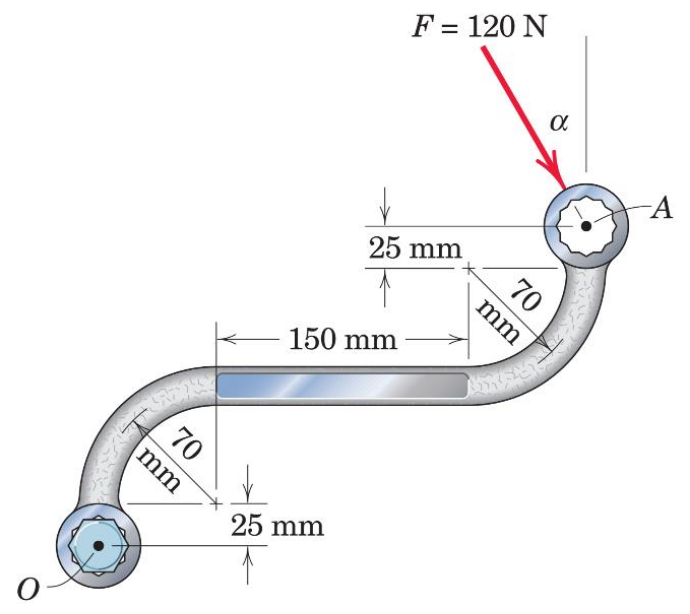
\includegraphics[width=0.5\textwidth]{problema.jpg}
\end{figure}

\end{problem}
\vspace{\baselineskip}

\end{document}
